
\documentclass[a4paper,10pt]{article}
\usepackage[utf8]{inputenc}
\usepackage[spanish]{babel}
\usepackage{amsmath}
\usepackage{amssymb}
\usepackage{amsfonts}
\usepackage{graphicx}
\spanishdecimal{.}


%opening
\title{Aprendizaje por refuerzo\\2023-II}
\author{Nombre: Emmanuel Peto Gutiérrez}
\date{\today}

\begin{document}

\maketitle

\paragraph{Instrucciones:} Para cada problema conteste lo que se le pide.

\begin{enumerate}
    \item (20 puntos)\textbf{Básico I: Explique lo siguiente}
    \begin{itemize}
        \item \textbf{(4 puntos) Describa los elementos de un problema de aprendizaje por refuerzo}
        
        \begin{itemize}
            \item \textit{Política:} Es lo que define cómo se debe comportar un agente en un punto del tiempo, dado el estado del ambiente.
            \item \textit{Señal de recompensa:} En cada paso que toma el agente, recibe un número del ambiente llamado \textit{recompensa} y el objetivo del agente es maximizar la recompensa total.
            \item \textit{Función de valor:} Ésta puede ser de estado o de acción. El valor de un estado es la recompensa esperada de un agente a lo largo del tiempo, dado que empieza en ese estado. En el caso de acción es la recompensa esperada dado que está en el estado $s$ y toma la acción $a$.
            \item \textit{Modelo:} Es algo que imita el comportamiento del ambiente. Permite hacer inferencias de cómo se va a comportar el ambiente.
        \end{itemize}
        
        \item \textbf{(4 puntos) ¿En qué se diferencia a un problema de aprendizaje supervisado o no supervisado?}
        
        En aprendizaje supervisado se busca resolver un problema de regresión o clasificación, donde se utiliza un conjunto de datos etiquetados para entrenar un modelo y se trata de predecir la etiqueta de un nuevo dato, usando el modelo entrenado. En aprendizaje no supervisado se trata de encontrar la estructura de un conjunto de datos no etiquetados, normalmente se utiliza para agrupar datos. Por otra parte, el objetivo del aprendizaje por refuerzo es maximizar una señal de recompensa y el agente utiliza la experiencia para tratar de obtener este objetivo.
        
        \item \textbf{(4 puntos) ¿Cuáles son los problemas centrales en aprendizaje por refuerzo?}
        
        Uno de los principales problemas es obtener un equilibrio entre exploración y explotación. Otro de los problemas es la incertidumbre que puede existir en el ambiente donde interactúa el agente.
        
        \item \textbf{(4 puntos) ¿Cuál es la diferencia entre los métodos en política y fuera de política?}
        
        Los métodos \textit{en política} intentan evaluar o mejorar la política que se ha usado para tomar decisiones. Los métodos \textit{fuera de política} evalúan o mejoran una política diferente de aquella usada para generar los datos.
        
        \item \textbf{(4 puntos) ¿Cuál es la diferencia entre los métodos de aprendizaje Q y gradiente de política?}
        
        Q-learning es un método fuera de política que aproxima directamente la función $q*$ (la función de acción-valor óptima) independientemente de la política que se siga, y a partir del valor estimado $q*$ se calcula la política $\pi *$. Por otra parte, los métodos de gradiente de política calculan una política parametrizada sin consultar una función de valor.
        
    \end{itemize}
    
    \item (20 puntos)\textbf{Programación dinámica: Usted se encuentra en un casino, tiene \$200.00 para este ejercicio y jugará hasta que pierda todo o hasta que duplique su dinero. Puede elegir entre dos juegos. El primero A, cuesta \$100.00 y da como retorno \$200.00 con probabilidad 0.05 y \$0.00 de lo contrario. El segundo B, cuesta \$200.00 y da como retorno \$300.00 con probabilidad 0.1 y \$0.00 de lo contrario. Hasta terminar, se elegirá jugar el juego A o B.}
   
Primero se modelará la situación con un autómata. El estado es la cantidad de dinero actual en mi bolsillo. La acción sería, dado que me alcanza el dinero, jugar $A$ o jugar $B$. La recompensa es -100 si pierdo todo, 0 en un estado intermedio y 100 si gano en total \$400.

\includegraphics[scale=1]{automata_casino}

    \begin{itemize}
	\item \textbf{(10 puntos) Provea un MDP que describa la situación}
	
	$\bullet$ Estados ($S$) = \{0, 100, 200, 300, 400\}
	
	$\bullet$ Acciones ($\mathcal{A}$) = \{$A$, $B$\}
	
	$\bullet$ Probabilidades ($p(s', r| s, a)$)
	
	\begin{tabular}{|c|c|c|c|c|}
	\hline
	$s'$ & $r$ & $s$ & $a$ & $p(s', r| s, a)$ \\ \hline
	0 & -100 & 100 & $A$ & 0.95 \\ \hline
	0 & -100 & 200 & $B$ & 0.9 \\ \hline
	100 & 0 & 200 & $A$ & 0.95 \\ \hline
	100 & 0 & 300 & $B$ & 0.9 \\ \hline
	200 & 0 & 100 & $A$ & 0.05 \\ \hline
	200 & 0 & 300 & $A$ & 0.95 \\ \hline
	300 & 0 & 200 & $A$ & 0.05 \\ \hline
	300 & 0 & 200 & $B$ & 0.1 \\ \hline
	400 & 100 & 300 & $A$ & 0.05 \\ \hline
	400 & 100 & 300 & $B$ & 0.1 \\ \hline
	\end{tabular}
	
	$\bullet$ Valor de descuento ($\gamma$): 1

	\item \textbf{(5 puntos) Aplique el algoritmo de iteración de valor para resolver el problema}
	
	Estos son los valores ($V$) obtenidos en 10 iteraciones:
	
	\begin{tabular}{|l|l|l|l|l|l|}
	\hline
	$it | S$ & 0 & 100 & 200 & 300 & 400 \\ \hline
	0 & 0 & 0 & 0 & 0 & 0 \\ \hline
        1 & 0 & -95.0 & -90.0 & -75.5 & 0 \\ \hline
        2 & 0 & -99.5 & -97.55 & -79.55 & 0 \\ \hline
        3 & 0 & -99.8775 & -97.955 & -79.88975 & 0 \\ \hline
        4 & 0 & -99.89775 & -97.988975 & -79.90797500000001 & 0 \\ \hline
        5 & 0 & -99.89944875 & -97.9907975 & -79.90950387500001 & 0 \\ \hline
        6 & 0 & -99.899539875 & -97.9909503875 & -79.9095858875 & 0 \\ \hline
        7 & 0 & -99.899547519375 & -97.99095858875 & -79.9095927674375 & 0 \\ \hline
        8 & 0 & -99.8995479294375 & -97.99095927674375 & -79.90959313649375 & 0 \\ \hline
        9 & 0 & -99.8995479638372 & -97.99095931364937 & -79.90959316745348 & 0 \\ \hline
        10 & 0 &-99.89954796568247 & -97.99095931674535 & -79.90959316911423 & 0 \\ \hline

	\end{tabular}
	
	\item \textbf{(5 puntos) ¿Cuál es la política óptima?}
	
	En la siguiente tabla se tienen los valores de $\sum_{s', r}p(s',r | s,a)[r + V(s')]$, para $a=A$ y $a=B$.
	
	\begin{tabular}{|l|l|l|l|}
	\hline
	    & 100 & 200 & 300 \\ \hline
	$A$ & -99.899 & -98.900 & -88.091 \\ \hline
        $B$ & null & -97.990 & -79.909 \\ \hline
	\end{tabular}
	
	De esta tabla se puede obtener la política óptima:
	
	\begin{tabular}{|c|c|}
	\hline
	$\pi (100)$ & $A$ \\ \hline
	$\pi (200)$ & $B$ \\ \hline
	$\pi (300)$ & $B$ \\ \hline
	\end{tabular}
	
    \end{itemize}

    \item \textbf{(15 puntos)\textbf{RL libre de modelo:} un agente explora un MDP $M=(S,A,R,P,\gamma)$ donde $S=\{s_1,s_2,s_3\}$ y $A=\{a_1,a_2,a_3\}$, $\gamma=0.5$ y $P(s,a_i,s_i)=1$ para cualquier $s$ para todo $i$. Las recompensas por transicionar a un estado son definidas como $R(s_i)=i$. La recompensa máxima es de 3.} 
    \begin{itemize}
	\item \textbf{(5 puntos) Dibuje en un diagrama el MDP propuesto}
	
	\includegraphics[scale=1]{mdp_qlearning}
	
	\item \textbf{(5 puntos) El agente sigue la trayectoria: $(s_1, a_1, 1, s_1 ,a_2, 2, s_2)$. Considere aprendizaje Q utilizando $\epsilon$-vóraz, donde una acción aleatoria nunca elije la acción vóraz, los empates se deciden eligiendo $a_i$ con la menor $i$. El factor de aprendizaje $\alpha=0.5$. Q se inicializa con ceros. ¿Podría el agente generar esa trayectoria para $\epsilon\neq 0$? de ser así, etiquete las acciones que son voraces y aquellas que son aleatorias}
	
	Sí es posible. Para ver cuales son las acciones voraces y cuales las aleatorias hay que ver la evolución de la matriz $Q$ a lo largo del episodio.
	
	matriz inicial:
	
	\[\begin{vmatrix}
        & a_1 & a_2 & a_3\\
        s_1 & 0 & 0 & 0\\
        s_2 & 0 & 0 & 0\\
        s_3 & 0 & 0 & 0\\
        \end{vmatrix}\]
        
        $s_1 \xrightarrow{a_1} s_1$: en esta transición se tomó la acción voraz, pero como todos son 0, se toma la de índice menor ($a_1$). Luego se actualiza la matriz
        
        $Q(s_1, a_1) = Q(s_1, a_1) + \alpha [R + \gamma \max_a Q(s_1, a) - Q(s_1, a_1)] = 0 + 0.5(1 + 0.5*0 - 0) = 0.5$
        \[\begin{vmatrix}
        & a_1 & a_2 & a_3\\
        s_1 & 0.5 & 0 & 0\\
        s_2 & 0 & 0 & 0\\
        s_3 & 0 & 0 & 0\\
        \end{vmatrix}\]
        
        $s_1 \xrightarrow{a_2} s_2$: en este punto la acción voraz para $s_1$ es $a_1$, por lo que se observa que se tomó una decisión aleatoria ($a_2$). Se actualiza la matriz
        
        $Q(s_1, a_1) = Q(s_1, a_1) + \alpha[R + \gamma \max_a Q(s_2, a) - Q(s_1, a_1)] = 0.5 + 0.5(2 + 0.5*0 - 0.5) = 1.25$
        
        \[\begin{vmatrix}
        & a_1 & a_2 & a_3\\
        s_1 & 1.25 & 0 & 0\\
        s_2 & 0 & 0 & 0\\
        s_3 & 0 & 0 & 0\\
        \end{vmatrix}\]
	
	\item \textbf{(5 puntos) Considere un algoritmo de inicialización llamado $Rmax$ donde todos los estados son inicializados con 6. ¿podría haber generado este método la trayectoria del inciso anterior? ¿por qué?}
    
    Al igual que en el inciso anterior, hay que observar la evolución de la matriz para ver si se puede o no.
    
    matriz inicial:
    
	\[\begin{vmatrix}
        & a_1 & a_2 & a_3\\
        s_1 & 6 & 6 & 6\\
        s_2 & 6 & 6 & 6\\
        s_3 & 6 & 6 & 6\\
        \end{vmatrix}\]
        
$s_1 \xrightarrow{a_1} s_1$: se tomó la acción voraz con índice menor ($a_1$).

$Q(s_1, a_1) = Q(s_1, a_1) + \alpha [R + \gamma \max_a Q(s_1, a) - Q(s_1, a_1)] = 6 + 0.5(1 + 0.5*6 - 6) = 5$
    \[\begin{vmatrix}
        & a_1 & a_2 & a_3\\
        s_1 & 5 & 6 & 6\\
        s_2 & 6 & 6 & 6\\
        s_3 & 6 & 6 & 6\\
        \end{vmatrix}\]

$s_1 \xrightarrow{a_2} s_2$: en este caso se tomó la acción voraz de índice menor $(a_2)$, por lo cual sí es posible que el agente genere esa trayectoria.

    \end{itemize}

    \item \textbf{(15 puntos)Aproximación de funciones:}
    \begin{itemize}
	\item \textbf{(5 puntos) Explique el algoritmo de DDQN y como se diferencia de DQN}
	
	Se describirá el algoritmo \textit{Double DQN}, pero dado que es una modificación de \textit{DQN} primero se explicará este.
	
	Luego, el algoritmo DQN es el siguiente:
	\begin{itemize}
	\item[1.] Inicializar los parámetros para $Q(s, a)$ y $\hat{Q}(s,a)$ con pesos aleatorios y un buffer de repetición vacío.
	\item[2.] Tomar una acción usando $\epsilon-$greedy.
	\item[3.] Ejecutar una acción $a$ y observar la recompensa, $r$, y el estado siguiente $s'$.
	\item[4.] Almacenar la transición $(s, a, r, s')$ en el buffer de repetición.
	\item[5.] Tomar un mini-lote aleatorio de las transiciones del buffer de repeticiones.
	\item[6.] Para cada transición en el buffer, calcula el objetivo $y=r$ si el episodio ya terminó en este paso, o $y=r+\gamma \max_{a' \in A} \hat{Q}(s', a')$ en otro caso.
	\item[7.] Calcula la pérdida $\mathcal{L} = (Q(s, a) - y)^2$
	\item[8.] Actualizar $Q(s, a)$ usando el algoritmo \texttt{SDG} minimizando la pérdida con respecto a los parámetros del modelo.
	\item[9.] Cada $N$ pasos, copiar los pesos de $Q$ a $\hat{Q}$
	\item[10.] Ir al paso 2 hasta que se cumpla una condición de convergencia. 
	\end{itemize}
	
	En el algoritmo \textit{Double DQN} simplemente se cambia la actualización de Bellman. En el DQN tradicional, el valor objetivo para $Q$ es el siguiente: \[Q(s_t, a_t) = r_t+\gamma \max_a Q'(s_{t+1}, a)\]
	
	En el algoritmo DDQN se eligen acciones para el siguiente estado usando la red entrenada, pero tomando valores de $Q$ de la red objetivo. La actualización de Bellman en este caso es \[Q(s_t, a_t) = r_t + \gamma \max_a Q' (s_{t+1}, argmax_a Q(s_{t+1}, a))\]
	
	La diferencia entre DDQN y DQN es que DQN sobreestima los valores de $Q$ y en algunos casos puede llevar a políticas subóptimas. El algoritmo Double DQN soluciona el problema de la sobreestimación.
	
	\item \textbf{(5 puntos) ¿Cuál es el rol de la repetición de experiencia? ¿en cuáles métodos se utiliza? ¿Cuál es la alternativa?}
	
	$\bullet$ La repetición de experiencia permite reducir la inestabilidad en el entrenamiento, ya que se toman lotes de experiencias aleatorias (tuplas, en este caso), donde cada experiencia tiene una baja probabilidad de estar correlacionada con otra en el mismo lote. 
	
	$\bullet$ Se utiliza en los método fuera de política.
	
	$\bullet$ Una alternativa para usar en métodos \textit{on-policy} es usar ambientes paralelos, todos ellos explotando la política actual.
	
	\item \textbf{(5 puntos)  Un ratón es involucrado en un experimento. Experimenta un episodio, en el primer paso escucha una campana. En el segundo paso ve una luz. En el tercer paso escucha una campana y ve una luz. Después recibe un pedazo de queso que vale 1 de recompensa y el episodio termina. Todas las otras recompensas fueron cero y el experimento no tiene descuento. Representar el estado del ratón $s$ por dos características $bell(s)\in{0,1}$ y $light(s)\in{0,1}$. Aplique el algoritmo de Q-learning para actualizar la tabla Q inicializanda en ceros.}
	
	Supongamos que un estado se representa mediante par ordenado $(b,l)$, donde $b$ es la variable que representa el estado de la campana y $l$ es la variable que representa el estado de la luz. Dado que las variables son binarias, hay 4 posibles estados. Supongamos que hay dos posibles acciones para cada estado: $n$: no hacer nada y $p$: dar un paso.
	
	\textbf{Nota:} se tomará la tasa de aprendizaje como $\alpha = 0.5$.
	
	La tabla $Q$ inicial sería la siguiente (una fila representa un estado y una columna una acción).
	
	\begin{tabular}{|c|c|c|}
	\hline
	   & $n$ & $p$ \\ \hline
	(0,0) & 0 & 0 \\ \hline
	(0,1) & 0 & 0 \\ \hline
	(1,0) & 0 & 0 \\ \hline
	(1,1) & 0 & 0 \\ \hline
	\end{tabular}
	
	$\bullet$ Paso 1: (0,0) $\xrightarrow{p}$ (1,0), $R = 0$
	
	$Q((0,0), p) = Q((0,0), p) + \alpha [R + \gamma \max_a Q((1,0), a) - Q((0,0), p)] = 0 + 0.5(0 + 1*0 - 0) = 0$
	
	Matriz después del paso 1:
	
	\begin{tabular}{|c|c|c|}
	\hline
	   & $n$ & $p$ \\ \hline
	(0,0) & 0 & 0 \\ \hline
	(0,1) & 0 & 0 \\ \hline
	(1,0) & 0 & 0 \\ \hline
	(1,1) & 0 & 0 \\ \hline
	\end{tabular}
	
	$\bullet$ Paso 2: (1,0) $\xrightarrow{p}$ (0,1), $R=0$
	
	$Q((1,0), p) = Q((1,0), p) + \alpha [R + \gamma \max_a Q((0,1), a) - Q((1,0), p)] = 0 + 0.5(0 + 1*0 - 0) = 0$
	
	Matriz después del paso 2:
	
	\begin{tabular}{|c|c|c|}
	\hline
	   & $n$ & $p$ \\ \hline
	(0,0) & 0 & 0 \\ \hline
	(0,1) & 0 & 0 \\ \hline
	(1,0) & 0 & 0 \\ \hline
	(1,1) & 0 & 0 \\ \hline
	\end{tabular}
	
	$\bullet$ Paso 3: (0,1) $\xrightarrow{p}$ (1,1), $R=1$
	
	$Q((0,1), p) = Q((0,1), p) + \alpha [1 + \gamma \max_a Q((1,1), a) - Q((0,1), p)] = 0 + 0.5(1 + 1*0 - 0) = 0.5$
	
	Matriz después del paso 3:
	
	\begin{tabular}{|c|c|c|}
	\hline
	   & $n$ & $p$ \\ \hline
	(0,0) & 0 & 0 \\ \hline
	(0,1) & 0 & 0.5 \\ \hline
	(1,0) & 0 & 0 \\ \hline
	(1,1) & 0 & 0 \\ \hline
	\end{tabular}
	
    \end{itemize}

    \item \textbf{(15 puntos)Exploración y explotación:}
    \begin{itemize}
	\item \textbf{(5 puntos) ¿Por qué es díficil el problema de exploración y explotación?}
	
	En una situación ideal, lo mejor sería realizar primero la exploración y cuando se tenga conocimiento del entorno completo, realizar explotación. Sin embargo, realizar sólo exploración primero puede tomar mucho tiempo, dado que el número de estados puede ser muy grande o incluso infinito (en el caso continuo). Por otra parte, si se realiza solamente explotación, se estaría tomando siempre la decisión que se cree óptima dado el conocimiento que se tiene hasta ahora, sin saber si otras no exploradas son mejores. Por eso, el aprendizaje por refuerzo trata de encontrar un equilibrio entre exploración y explotación tomando decisiones no deterministas (como $\epsilon$-greedy).
	
	\item \textbf{(5 puntos) ¿Describa el método de UCB?}
	
	\emph{Upper-confidence-bound} estima la confianza superior para cada valor-acción. Es un método que selecciona una acción de acuerdo a su potencial de ser óptima. La acción $A_t$ se selecciona de acuerdo a la siguiente fórmula \[A_t = argmax_a [Q_t(a) +c \sqrt{\frac{\ln t}{N_t(a)}}] \] donde $t$ es el tiempo y $N_t(a)$ es el número de veces que ha sido seleccionada la acción $a$ hasta el tiempo $t$.
	
	\item \textbf{(5 puntos) Suponga que tenemos un problema de bandido multi-brazo donde existen 3 acciones disponibles. Siguiendo el principio de optimismo bajo incertidumbre, ¿Cuáles serían las primeras 4 acciones a tomar? y ¿por qué?}
	
	Este principio favorece la exploración, seleccionando aquella acción en donde existe mayor incertidumbre. Para este caso, entre menos veces haya sido seleccionada una acción, mayor incertidumbre tendrá; y si hay empates se selecciona la acción de menor índice. Supongamos que las acciones están indexadas: $a_1$, $a_2$ y $a_3$. Como al principio las 3 han sido seleccionadas 0 veces, entonces existe la misma incertidumbre en las tres y se selecciona $a_1$. En la segunda se selecciona $a_2$ y en la tercera $a_3$. En este punto las 3 han sido seleccionadas exactamente una vez, por lo que tienen la misma incertidumbre, así que en la cuarta selección se elige a la de índice menor ($a_1$).
	
	Las primeras 4 acciones se seleccionan en el siguiente orden: $a_1$, $a_2$, $a_3$ y $a_4$.
	
    \end{itemize}

    \item \textbf{(15 puntos)Temas avanzados:}
    \begin{itemize}
	   \item \textbf{(5 puntos) Considere el siguiente problema y utilice el método de métricas ponderada con $w=[0.5,0.5]^T$, $p=2$ y encontrar el óptimo} $$\min_{x\in[-10,10]^2} (x_1^2+x_2^2, (x_1-5)^2+(x_2-5)^2)$$
	   
	   El método de la suma ponderada trata de minimizar la siguiente función $w \cdot f(x_1, x_2) = \sum w_i f_i$. Primero se obtiene la función $g(x_1, x_2) = w \cdot f$\\
	   $ = 0.5(x_1^2 + x_2^2) + 0.5((x_1-5)^2 + (x_2-5)^2)$\\
	   $ = 0.5x_1^2 + 0.5x_2^2 + 0.5x_1^2 - 5x_1+12.5+0.5x_2^2-5x_2+12.5$\\
	   $ = x_1^2 + x_2^2 - 5x_1 - 5x_2 + 25$
	   
	   Se calculan las derivadas parciales y se igualan a 0 para encontrar el punto $(x_1, x_2)$ donde se encuentra el mínimo de $g(x_1, x_2)$.
	   
	   $\frac{\partial g}{\partial x_1} = 2x_1 - 5 = 0$\\
	   $\Rightarrow x_1 = 2.5$
	   
	   De manera análoga se puede encontrar $x_2 = 2.5$
	   
	   Así, la función $g$ evaluada en el punto (2.5, 2.5) es:\\
	   $2.5^2 + 2.5^2 -5(2.5) - 5(2.5) + 25$\\
	   $=12.5$
	   
	   El cual es el valor óptimo.
	   
  	  \item \textbf{(5 puntos) Lea y critique el siguiente artículo CS de Witt et al. (2020). Deep Multi-Agent Reinforcement Learning for Decentralized Continuous Cooperative Control}
  	  
  	  El artículo habla de diferentes herramientas de aprendizaje por refuerzo, multiagente, en un ambiente continuo. Ponen a prueba las diferentes herramientas en ambientes de robots multi-agente y el ambiente depredador-presa, donde al final grafican y comparan los resultados. Al principio se habla sobre control en robots y se mencionan benchmarks que se utilizan para esto. Una forma de hacer control multi-agente sobre un solo robot es descomponerlo en diferentes segmentos y cada agente controla un segmento.
  	  
  	  $\bullet$ \textit{Los antecedentes}
  	  
  	  Antes de hablar del experimento se dan los antecedentes, donde se muestran definiciones. Los experimentos se llevan a cabo en una tarea completamente cooperativa, multi-agente, en la cual un equipo de agentes cooperativos toman acciones secuenciales en un ambiente parcialmente observable. Se explican los diferentes métodos de aprendizaje que se usaron en el experimento, como DQN, VDN, QMIX y MADDPG.
  	  
  	  $\bullet$ \textit{Mujoco}
  	  
  	  En esta sección se explica el funcionamiento del benchmark \textit{Mujoco}, el cual se utiliza para hacer control descentralizado cooperativo multi-agente sobre robots. Se crearon escenarios en los que multiples agentes tienen que resolver una tarea de forma cooperativa, partiendo un robot en varias partes y cada agente controlado una parte.
  	  
  	  $\bullet$ \textit{COMIX y FacMADDPG}
  	  
  	  Se explican otros dos algoritmos multi-agente. COMIX se basa en Q-learning mientras que FacMADDPG se basa en gradiente de política.
  	  
  	  $\bullet$ \textit{Preparación del experimento}
  	  
  	  En esta parte se describen las características de los experimentos presa-depredador multi-agente, donde los agentes son los depredadores, y los robots muti-agente de Mujoco. También se habla de cómo se evalúa el desempeño de cada método en estos ambientes.
  	  
  	  $\bullet$ \textit{Resultados}
  	  
  	  En la última parte se muestran las gráficas de resultados donde se comparan los métodos COMIX, FacMADDPG, MADDPG y COVDN. En las gráficas se observa el valor de retorno de cada método respecto a los pasos del ambiente. Los métodos se evalúan en 4 ambientes diferentes: depredador-presa, 2-Agent HalfCheeta, 2-Agent walker y 3-Agent Hopper; siendo los 3 últimos los robots del benchmark Mujoco.
	  
	  \item \textbf{(5 puntos) Lea y critique el siguiente artículo A Mahajan et al. (2022). Generalization in Cooperative Multi-Agent Systems}
	  
	  El artículo habla de sistemas cooperativos multi-agente. Específicamente, se habla del problema de la generalización combinatoria, en el cual se tiene un ambiente en el que puede cambiar el número de agentes o las habilidades. En la introducción se ejemplifica el problema con un partido de fútbol, en el que pueden cambiar a los jugadores, existe incertidumbre sobre las habilidades de otros jugadores y cada jugador tiene un rol.
	  
	  $\bullet$ \textit{Antecedentes}
	  
	  Se modela la tarea multi-agente cooperativo como un MDP parcialmente observable descentralizado. Se describe con fórmulas matemáticas al MDP.
	  
	  $\bullet$ \textit{Análisis}
	  
	  En esta sección se dan todos los teoremas y corolarios para caracterizar a las variables del MDP.
	  
	  $\bullet$ \textit{Preparación del experimento}
	  
	  Se describen los diferentes ambientes donde se ponen a prueba los algoritmos MARL. Los ambientes son:
	  \begin{itemize}
	  \item fruit forage
	  \item predator prey
	  \item StrarCraft II
	  \end{itemize}
	  
	  $\bullet$ \textit{Resultados}
	  
	  Finalmente, se grafican y se comparan los resultados de diferentes métodos multi-agente cooperativo. Los métodos que se comparan son QMIX, VDN, IPPO, MAPPO.
	  
    \end{itemize}

\end{enumerate}

\end{document}

